\documentclass[12pt]{article}
\usepackage{geometry} % see geometry.pdf on how to lay out the page. There's lots.
\geometry{a4paper} % or letter or a5paper or ... etc

\usepackage{graphicx,url}
%\usepackage[brazil]{babel}   
\usepackage[latin1]{inputenc}  

%stuff for maths
\usepackage{amssymb} %maths
\usepackage{amsmath} %maths
\providecommand{\abs}[1]{\lvert#1\rvert}
%\usepackage[utf8]{inputenc} %useful to type directly diacritic characters


\sloppy

\title{Imaging Transforms from the Ambisonic Toolkit:\\
	a new approach to sound-image composition}

\author{Joseph Anderson}
\date{} % delete this line to display the current date

%\author{Joseph Anderson\inst{1}}

%\address{School of Arts \& New Media --
%         University of Hull \\
%         Scarborough Campus -- Scarborough, United Kingdom
%         \email{j.anderson@hull.ac.uk}
%}


\begin{document}

\maketitle

\begin{abstract}
  Make a nice abstract. [re-write]
\end{abstract}

%\begin{abstract}
%  This meta-paper describes the style to be used in articles and short
%  papers for SBC conferences. For papers in English, you should add
%  just an abstract, and for papers in Portuguese, we also ask for
%  an abstract in Portuguese (``resumo''). In both cases, abstracts
%  should not have more than 10 lines and must be in the first page of
%  the paper.
%\end{abstract}


%\section{General Information}\label{sec:gen}

%writing starts here
\section{Introduction}

The Ambisonic Tool Kit (ATK) is intended to bring together a number of tools and transforms for working with Ambisonic surround sound. Rather than focusing on the needs and concerns of the classical music sound recordist or the popular music mix-engineer/producer or the acoustician/engineer, use is targeted towards the composer of acousmatic music. The intention is for the toolset to be both ergonomic and comprehensive, providing algorithms to creatively manipulate and synthesize Ambisonic soundfields.

The tools are framed for the user to `think Ambisonically'. By this, it is meant the ATK is not focused on the problem of auralization and/or room modelling. Auralization is a complex problem beyond the scope of the fundamental algorithms of the ATK. (It is worth noting, however, with the toolset provided, successful room modelling may be implemented.) Interestingly enough, many composers of acousmatic music often do not move beyond the problem of auralization or room modelling. The ATK, by addressing the holistic problem of creatively controlling a complete soundfield allows and encourages the composer to think beyond the placement of sounds in a sound-space and instead attend to the impression and image of a soundfield, therefore taking advantage of the model the Ambisonic technology presents. This is viewed to be the {\em idiomatic} approach for working with the Ambisonic technique.

Restated, the model of the ATK is a sound-field sound-image model rather than a sound-object sound-scene model.

The remainder of this document is divided into sections detailing the elements of the toolset. These are encoders, transforms, and decoders. At present the ATK is limited to `canonical' 1st-order B-format only. Work in higher orders is a topic of current research in the field. In particular, suitable dominance transforms are currently un-realised.


\subsection{Weightings}

Describe weighting scheme.

There's an argument to me made as to whether we should use `canonical' W, \(\frac{1}{\sqrt{2}}\), `unscaled', 1, `normalised', \(\frac{1}{\sqrt{3}}\), or other, e.g., {\em SND3}. The Graz Ambisonic community has posed this as a point of question.

\subsection{HOA}

HOA issues.

\section{Encoding}

\subsection{Point Source}

Point source panner.

%need to come up with some custom stuff, so that there is a macro for name and interface
Algorithm name: Mono to B

\begin{equation}	\label{eq:point_encode}
\mathbf{S}_{\theta, \phi} = \begin{pmatrix}
	\frac{1}{\sqrt{2}}\\
	\cos{\phi} \cos{\theta}\\
	\cos{\phi} \sin{\theta}\\
	\sin{\phi}
\end{pmatrix}
\end{equation}


\subsection{Point Source with Focus}

Point source panner.\footnote{Mention Menzies W-format and O-format.}

%need to come up with some custom stuff, so that there is a macro for name and interface
Algorithm\footnote{Algorithm is focus followed by elevate, rotate.} name: ??

\begin{equation}	\label{eq:point_encode}
\mathbf{S}_{\theta, \phi, \alpha} = \frac{1}{1 + \sin{\abs{\alpha}}} \begin{pmatrix}
	\frac{1}{\sqrt{2}}\\
	\cos{\phi} \cos{\theta} \sin{\alpha}\\
	\cos{\phi} \sin{\theta} \sin{\alpha}\\
	\sin{\phi} \sin{\alpha}
\end{pmatrix}
\end{equation}


\subsection{Stereo}

\begin{equation}	\label{eq:stereo_sig}
A_{LR} = \begin{pmatrix}
	L\\
	R
\end{pmatrix}
\end{equation}

\begin{equation}	\label{eq:ms_matrix}
\mathbf{S}_{MS} = \begin{pmatrix}
	\frac{1}{\sqrt{2}} & \frac{1}{\sqrt{2}} \\
	\frac{1}{\sqrt{2}} & -\frac{1}{\sqrt{2}}
\end{pmatrix}
\end{equation}


\subsubsection{SimpleStereo}


%\begin{equation}	\label{eq:simple_stereo}
%\mathbf{S}_{Z, \alpha} = \begin{pmatrix}
%	\frac{1}{\sqrt{2}} & \frac{1}{\sqrt{2}} \\
%	\sin{\alpha} & \sin{\alpha}\\
%	\cos{\alpha} & -\cos{\alpha}\\
%	0 & 0
%\end{pmatrix}
%\end{equation}

\begin{equation}	\label{eq:simple_stereo}
\mathbf{S}_{Z, \alpha} = \begin{pmatrix}
	\frac{1}{\sqrt{2}} & 0 \\
	\sin{\alpha} & 0\\
	0 & \cos{\alpha}\\
	0 & 0
\end{pmatrix}
\end{equation}


\(\alpha\) is the distortion angle, or {\em focus}.


\subsubsection{SuperStereo}

Name\footnote{At the moment, named as `Stereo to B' in Python ATK.} 

Include network diagram? Include Hilbert transform? Include a reference to algorithm and the private email discussion on phasiness with Geoff Barton and Martin Leese. The below algorithm includes `forward preference'.

\(j = \sqrt{-1}\), \(w\) is width, \(a\) is phasiness, `forward preference'.

%\begin{equation}	\label{eq:super_stereo}
%\mathbf{S}_{Z, \alpha} = \begin{pmatrix}
%	c_{0} - c_{1}wj & c_{0} + c_{1}wj \\
%	c_{2} + c_{3}wj & c_{2} - c_{3}wj\\
%	(c_{4} + c_{5}a )w - (c_{6} -  c_{7}a)j & -(c_{4} + c_{5}a )w - (c_{6} -  c_{7}a)j\\
%	0 & 0
%\end{pmatrix}
%\end{equation}

\begin{equation}	\label{eq:super_stereo}
\mathbf{S}_{Z, \alpha} = \begin{pmatrix}
	c_{0} & -c_{1}wj \\
	c_{2} &  c_{3}wj\\
	- (c_{4} -  c_{5}a)j & (c_{6} + c_{7}a)w\\
	0 & 0
\end{pmatrix}
\end{equation}


\begin{equation}
	c_{0} = 0.6098637
\end{equation}
\begin{equation}
	c_{1} = 0.6896511
\end{equation}
\begin{equation}
	c_{2} = 0.8624776
\end{equation}
\begin{equation}
	c_{3} = 0.7626955
\end{equation}
\begin{equation}
	c_{4} = 0.2156194
\end{equation}
\begin{equation}
	c_{5} = 0.6098637
\end{equation}
\begin{equation}
	c_{6} = 1.6822415
\end{equation}
\begin{equation}
	c_{7} = 0.6896511
\end{equation}



\subsection{Soundfield (A-B)}

A-B matricies. Need to describe algorithm for weightings.

Also, consider adding tetrahedrons to illustrate, and/or plots.

Matrices are arranged so that `maximum scattering' pairs are adjacent.

%Need to come up with a naming scheme for the matrices!!!
\subsubsection{Front Left Up}


\begin{equation}	\label{eq:aflu_sig}
A_{FLU} = \begin{pmatrix}
	FLU\\
	FRD\\
	BLD\\
	BRU
\end{pmatrix}
\end{equation}

\begin{equation}	\label{eq:ab_flu}
\mathbf{S}_{FLU} = \frac{1}{2} \begin{pmatrix}
	1 & 1 & 1 & 1\\
	1 & 1 & -1 & -1\\
	1 & -1 & 1 & -1\\
	1 & -1 & -1 & 1
\end{pmatrix}
\end{equation}

\subsubsection{Front Left Down}

\begin{equation}	\label{eq:afld_sig}
A_{FLD} = \begin{pmatrix}
	FLD\\
	FRU\\
	BLU\\
	BRD
\end{pmatrix}
\end{equation}


\begin{equation}	\label{eq:ab_fld}
\mathbf{S}_{FLD} = \frac{1}{2} \begin{pmatrix}
	1 & 1 & 1 & 1\\
	1 & 1 & -1 & -1\\
	1 & -1 & 1 & -1\\
	-1 & 1 & 1 & -1
\end{pmatrix}
\end{equation}

\subsubsection{Front Left-Right}

\begin{equation}	\label{eq:aflr_sig}
A_{FLR} = \begin{pmatrix}
	FL\\
	FR\\
	BU\\
	BD
\end{pmatrix}
\end{equation}


\begin{equation}	\label{eq:ab_flr}
\mathbf{S}_{FLR} = \frac{1}{2} \begin{pmatrix}
	1 & 1 & 1 & 1\\
	1 & 1 & -1 & -1\\
	\sqrt{2} & -\sqrt{2} & 0 & 0\\
	0 & 0 & \sqrt{2} & -\sqrt{2}
\end{pmatrix}
\end{equation}

\subsubsection{Front Up-Down}

\begin{equation}	\label{eq:afud_sig}
A_{FUD} = \begin{pmatrix}
	FU\\
	FD\\
	BL\\
	BR
\end{pmatrix}
\end{equation}

\begin{equation}	\label{eq:ab_fud}
\mathbf{S}_{FUD} = \frac{1}{2} \begin{pmatrix}
	1 & 1 & 1 & 1\\
	1 & 1 & -1 & -1\\
	0 & 0 & \sqrt{2} & -\sqrt{2}\\
	\sqrt{2} & -\sqrt{2} & 0 & 0
\end{pmatrix}
\end{equation}

\subsubsection{Front \& Back Up}

\begin{equation}	\label{eq:afbu_sig}
A_{FBU} = \begin{pmatrix}
	F\\
	BU\\
	BLD\\
	BRD
\end{pmatrix}
\end{equation}


\begin{equation}	\label{eq:ab_fbu}
\mathbf{S}_{FBU} = \frac{1}{2} \begin{pmatrix}
	1 & 1 & 1 & 1\\
	\sqrt{3} & -\frac{1}{\sqrt{3}} & -\frac{1}{\sqrt{3}} & -\frac{1}{\sqrt{3}}\\
	0 & 0 & \sqrt{2} & -\sqrt{2}\\
	0 & 2\frac{\sqrt{2}}{\sqrt{3}} & -\frac{\sqrt{2}}{\sqrt{3}} & -\frac{\sqrt{2}}{\sqrt{3}}
\end{pmatrix}
\end{equation}

\subsubsection{Front Left-Right Up}

\begin{equation}	\label{eq:aflru_sig}
A_{FLRU} = \begin{pmatrix}
	FLU\\
	FRU\\
	FD\\
	B
\end{pmatrix}
\end{equation}

\begin{equation}	\label{eq:ab_flru}
\mathbf{S}_{FLRU} = \frac{1}{2} \begin{pmatrix}
	1 & 1 & 1 & 1\\
	\frac{1}{\sqrt{3}} & \frac{1}{\sqrt{3}} & \frac{1}{\sqrt{3}} & -\sqrt{3}\\
	\sqrt{2} & -\sqrt{2} & 0 & 0\\
	\frac{\sqrt{2}}{\sqrt{3}} & \frac{\sqrt{2}}{\sqrt{3}} & -2\frac{\sqrt{2}}{\sqrt{3}} & 0 
\end{pmatrix}
\end{equation}


\subsubsection{Front \& Back Down}

\begin{equation}	\label{eq:afbd_sig}
A_{FBD} = \begin{pmatrix}
	F\\
	BD\\
	BLU\\
	BRU
\end{pmatrix}
\end{equation}


\begin{equation}	\label{eq:ab_fbd}
\mathbf{S}_{FBD} = \frac{1}{2} \begin{pmatrix}
	1 & 1 & 1 & 1\\
	\sqrt{3} & -\frac{1}{\sqrt{3}} & -\frac{1}{\sqrt{3}} & -\frac{1}{\sqrt{3}}\\
	0 & 0 & \sqrt{2} & -\sqrt{2}\\
	0 & -2\frac{\sqrt{2}}{\sqrt{3}} & \frac{\sqrt{2}}{\sqrt{3}} & \frac{\sqrt{2}}{\sqrt{3}}
\end{pmatrix}
\end{equation}

\subsubsection{Front Left-Right Down}

\begin{equation}	\label{eq:aflrd_sig}
A_{FLRD} = \begin{pmatrix}
	FLD\\
	FRD\\
	FU\\
	B
\end{pmatrix}
\end{equation}


\begin{equation}	\label{eq:ab_flrd}
\mathbf{S}_{FLRD} = \frac{1}{2} \begin{pmatrix}
	1 & 1 & 1 & 1\\
	\frac{1}{\sqrt{3}} & \frac{1}{\sqrt{3}} & \frac{1}{\sqrt{3}} & -\sqrt{3}\\
	\sqrt{2} & -\sqrt{2} & 0 & 0\\
	-\frac{\sqrt{2}}{\sqrt{3}} & -\frac{\sqrt{2}}{\sqrt{3}} & 2\frac{\sqrt{2}}{\sqrt{3}} & 0 
\end{pmatrix}
\end{equation}


\subsection{Special}

Other, known, special arrays. This may be expanded to include a number of `standard' surround arrays. (Though, the A to B encodings are preferred in many cases.)

\subsubsection{ZoomH2}


%need to come up with some custom stuff, so that there is a macro for name and interface
Algorithm name: ZoomH2 to B

Ideally this needs filtering to compensate for poor capsule response and layout. Also need to check that the expressed matrix results in correct matrix! The scaling matrix could be in the wrong place!!


\begin{equation}	\label{eq:azoomh2_sig}
A_{FBD} = \begin{pmatrix}
	FL\\
	FR\\
	BL\\
	BR
\end{pmatrix}
\end{equation}


\begin{equation}	\label{eq:zoomh2}
\mathbf{S}_{ZoomH2} = 2 \begin{pmatrix}
	\frac{1}{2 \sqrt{2} + 2}\\
	\frac{1}{\sqrt{2} + 1}\\
	\frac{1}{\sqrt{2} + \sqrt{3}}\\
	0
\end{pmatrix} \begin{pmatrix}
	1 & 1 & \sqrt{2} & \sqrt{2}\\
	1 & 1 & -1 & -1\\
	1 & -1 & 1 & -1\\
	0 & 0 & 0 & 0
\end{pmatrix}
\end{equation}

%	\frac{1}{\sqrt{2} + 2} & \frac{1}{\sqrt{2} + 2} & \frac{1}{\sqrt{2} + 2} & \frac{1}{\sqrt{2} + 2} \\


\section{Soundfield Transforms}

Describe soundfield transforms here, as does Chapman. Rotation, mirroring, dominance


\begin{equation}	\label{eq:trans}
	B^\prime = \mathbf{T} B
\end{equation}

\section{Rotations}

Text.

\subsection{Rotate}

\begin{equation}	\label{eq:rotate}
\mathbf{R}_{Z, \theta} = \begin{pmatrix}
	1 & 0 & 0 & 0\\
	0 & \cos{\theta} & -\sin{\theta} & 0\\
	0 & \sin{\theta} & \cos{\theta} & 0\\
	0 & 0 & 0 & 1
\end{pmatrix}
\end{equation}

\subsection{Tilt}

\begin{equation}	\label{eq:tilt}
\mathbf{R}_{X, \phi} = \begin{pmatrix}
	1 & 0 & 0 & 0\\
	0 & 1 & 0 & 0\\
	0 & 0& \cos{\phi} & -\sin{\phi}\\
	0 & 0& \sin{\phi} & \cos{\phi}
\end{pmatrix}
\end{equation}

\subsection{Tumble}

\begin{equation}	\label{eq:tumble}
\mathbf{R}_{Y, \phi} = \begin{pmatrix}
	1 & 0 & 0 & 0\\
	0 & \cos{\phi}  & 0 & -\sin{\phi}\\
	0 & 0 & 1 & 0\\
	0 & \sin{\phi}  & 0 & \cos{\phi}
\end{pmatrix}
\end{equation}

\section{Dominance and variants}
\label{sec:dominance}

In his report to the UK's National Research Development Corporation (NRDC) \cite{gerzon:75a} Gerzon introduced {\em dominance} as a useful and creative transform to apply to ambisonic soundfields. The initial applications proposed appear to focus on the needs of the audio engineer, and are discussed as if the engineer is working to post-process B-format concert recordings made with a soundfield microphone \cite{farrar:79}. In his NRDC report Gerzon describes dominance as a {\em width} control: \begin{quote}
[Which] permits the relative width of the front and back images to be varied (e.g. to modify the width of an orchestra or to emphasise the rear reverberation).... [P]lus an up/down width control that, for example, allows a below-horizontal orchestra and audience (caused by high-up microphones) to be made horizontal by narrowing the upward width.
\end{quote} Here Gerzon is describing the action of dominance\footnote{Menzies \cite{menzies:99} has given a somewhat more detailed and precise description: Dominance has the effect of moving the directions towards or away from a special direction, the {\em direction of the dominance}. If the {\em dominance factor} is zero, then it [is] the identity. At maximum dominance the directions are all changed to the direction of dominance. Associated with the change of directions is a gain factor. For initial directions further from the dominance direction, the gain is relatively less than for closer directions. At maximum dominance opposed directions are eliminated completely by zero gain. Dominance has been used as a kind of zooming tool to give gain emphasis locally while maintaining B-format integrity. }, firstly on the \(X\) axis and then on the \(Z\) axis. The dominance transform on the \(X\) axis is represented in his report as \begin{equation}	\label{eq:mu_dom}
\mathbf{Z}_{X, \mu} = \begin{pmatrix}
	1 & \frac{1}{\sqrt{2}}\mu & 0 & 0\\
	\sqrt{2}\mu & 1 & 0\\
	0 & 0 & \sqrt{1-\mu^2} & 0\\
	0 & 0 & 0 & \sqrt{1-\mu^2}
\end{pmatrix}
\end{equation} where \(\mu\) conveniently controls the amount of dominance applied. Valid values for \(\mu\) are \begin{equation}
-1 \leq \mu \leq 1
\end{equation} When \(\mu = 1\), maximum dominance in the forward direction is applied, with the resulting soundfield compressed to a point source (mono) image at front-centre. As well as spatial distortions, gains are also varied. The gain of what was previously encoded in the input B-format signal at front-centre is increased by \(+6\) dB, and at back-centre gain is reduced to \(-\infty\) dB. Elements on the \(Y \textendash Z\) plane retain their previous gains. The astute observer will recognise this is equivalent to placing a single cardioid microphone in the soundfield aimed at front-centre, increasing the gain by \(+6\) dB, and then re-encoding this mono signal into a new B-format signal as a point source image at front-centre (\(\theta, \phi = 0\textdegree, 0\textdegree\)).

Dominance can also be represented in terms of gain applied in the direction of dominance. Gerzon and Barton \cite{gerzon-barton:92} have illustrated this form as follows \begin{equation}
\mathbf{D}_{X, \lambda} = \begin{pmatrix}		\label{eq:lamb_dom}
	\frac{1}{2}(\lambda + \frac{1}{\lambda}) & \frac{1}{\sqrt{8}}(\lambda - \frac{1}{\lambda}) & 0 & 0\\
	\frac{1}{\sqrt{2}}(\lambda - \frac{1}{\lambda}) & \frac{1}{2}(\lambda + \frac{1}{\lambda}) & 0 & 0\\
	0 & 0 & 1 & 0\\
	0 & 0 & 0 & 1
\end{pmatrix}
\end{equation} where \(\lambda\) controls dominance as gain applied at front-centre. If \(\lambda\) is defined as \begin{equation}
	\lambda = 10^\frac{g}{20}
\end{equation} \(g\) controls dominance as gain in dB applied at front-centre. The gain at back-center will be equal to \(-g\) dB. Figure~\ref{fig:dominanceFig} illustrates gain and angular distortions applied to a B-format soundfield with varying values of \(g\). This is the dominance variant named in the Ambisonic Toolkit as {\em dominance}.

These two forms of dominance have appeared throughout the literature named as both {\em dominance} and {\em zoom}.\footnote{Below we'll seek to address this naming issue further.} Malham \cite{malham:90} has shown how these two variants may be regarded as equivalent, with further discussion to be found elsewhere in the literature \cite{daniel:01} \cite{hollerweger:06}. From a user point of view, however, varying \(\mu\) gives a different experience of manipulating the soundfield than does varying \(g\). For example, we've seen that for the dominance variant presented in \eqref{eq:mu_dom}, \(\mu = 1\) gives maximum dominance, with the image collapsing to a point source image at front-centre. To achieve the equivalent spatial distortion with \eqref{eq:lamb_dom} requires \(g= \infty\) dB. As you'd imagine, this is not particularly ideal. In practice, then, we'd expect that at least two forms of dominance to be desirable. Below we'll present two further variants which have been deemed to be musically useful,\footnote{And appear in the Ambisonic Toolkit.} along with other derived transforms developed to address features of dominance that may be regarded as less suitable in some circumstances.


%\subsection{Dominance}

\subsection{Zoom}

Both \eqref{eq:mu_dom} and \eqref{eq:lamb_dom} have been described as both dominance and zoom, which can lead to some confusion. In practice, it appears that \eqref{eq:mu_dom} is usually described as zoom. Within the Ambisonic Toolkit, we'll use this form, but instead apply dominance as a {\em dominance angle of distortion}, \(\alpha\).\footnote{The form presented here varies from that presented in \cite{anderson:09a}, which is derived from \eqref{eq:lamb_dom}.} The rationale for this being to supply a dominance variant that matches previous practice (under the name of zoom), yet provides slightly different, but musically useful, ergonomics.\footnote{Additionally we'll also see that further imaging transforms are supplied in terms of \(\alpha\).}

The ATK's zoom applies \eqref{eq:mu_dom}, but in terms of a distortion angle \(\alpha\), with valid values \begin{equation}
	-90\textdegree \leq \alpha \leq 90\textdegree
\end{equation} giving the user the option of directly considering dominance in terms of angular distortions. Daniel \cite{daniel:01} has conveniently shown how \eqref{eq:mu_dom} transforms the angles (in the \(X-Y\) plane) of an input sounfield in terms of \(\mu\):

\begin{equation}		\label{eq:daniel_1}
	cos\theta^\prime = \frac{\mu + cos\theta}{1 +\mu cos\theta}
\end{equation}The original encoded angle of incidence in the \(X-Y\) plane is \(\theta\) and the resulting transformed angle is \(\theta^\prime\). We can consider what happens to the sound encoded at the hard-left of the image by setting \(\theta = 90\textdegree\). Equation \eqref{eq:daniel_1} then simplies to: \begin{equation}		\label{eq:daniel_2}
	cos\theta^\prime = \mu
\end{equation} Describing \(\theta^\prime\) in terms of the dominance angle of distortion, \(\alpha\) \begin{equation}
	\theta^\prime = 90\textdegree - \alpha
\end{equation} and with further simplification and substitution \eqref{eq:mu_dom} becomes\begin{equation}	\label{eq:zoom}
\mathbf{Z}_{X, \alpha} = \begin{pmatrix}
	1 & \frac{1}{\sqrt{2}}\sin{\alpha} & 0 & 0\\
	\sqrt{2}\sin{\alpha} & 1 & 0 & 0\\
	0 & 0 & \cos{\alpha} & 0\\
	0 & 0 & 0 & \cos{\alpha}
\end{pmatrix}
\end{equation} which is the transform the ATK names as zoom. Figure~\ref{fig:zoomFig} illustrates gain and angular distortions applied to a B-format soundfield as zoom is applied in terms of \(\alpha\). 

\subsubsection{Balance}

We've seen Gerzon describe the dominance (zoom) transform as being akin to a width transform.\footnote{The author has described a number of classic two-channel stereo transforms in \cite{anderson:09b}.} Applying zoom in the form of \eqref{eq:zoom} on the \(Y\) axis results in a transform having a similar result to the well known stereo {\em balance} transform. The ATK's balance is shown here \begin{equation}	\label{eq:balance}
\mathbf{Z}_{Y, \alpha} = \begin{pmatrix}
	1 & 0 & \frac{1}{\sqrt{2}}\sin{\alpha} & 0\\
	0 & \cos{\alpha} & 0 & 0\\
	\sqrt{2}\sin{\alpha} & 0 & 1 & 0\\
	0 & 0 & 0 & \cos{\alpha}
\end{pmatrix}
\end{equation} with valid values \begin{equation}
	-90\textdegree \leq \alpha \leq 90\textdegree
\end{equation} Distortion angle \(\alpha\) controls the displacement of both front-centre and back-center, where \(\alpha = 90\textdegree\) pushes the image to hard-left, \(\alpha = -90\textdegree\) to hard-right, and \(\alpha = 0\textdegree\) leaves the image untouched. Figure~\ref{fig:balanceFig} illustrates the results the effect of balance with positive values of \(\alpha\).


\subsection{Focus}

Daniel \cite{daniel:01} has described a transform he names as {\em focus}:  \begin{quote} ... implemented by V\'{e}ronique Larcher for [a] work [of] spatial sound composition [by] C\'{e}cile le Prado.\footnote{Name the piece or pieces here. Emailed V\'{e}ronique with the question.} The visual analogue approximate [to] the effect of a flashlight scanning the darkness.\footnote{Translation: http://translate.google.co.uk}
\end{quote} To realise this effect he advises using \eqref{eq:mu_dom}, setting \(\mu = 0\). The results are as described previously in the introduction to section \ref{sec:dominance}.

The ATK takes a slightly different approach, preferring for imaging transforms to be continuously variable. Instead we take the zoom transform of \eqref{eq:zoom} and normalise gain in the direction zoom is applied, so that at maximum zoom, \(\alpha =  90\textdegree\), the gain is \(0\) dB rather than \(+6\) dB as in \eqref{eq:zoom}. For zoom, gain in the direction of applied dominance is \begin{equation}
	1 + \sin{\alpha}
\end{equation} If we wish our gain normalisation to behave well for both positive and negative values of \(\alpha\), so that gain in normalised in the direction focus is applied, we'll need to use \begin{equation}		\label{eq:foc_norm}
	1 + \sin{\abs{\alpha}}
\end{equation} Normalising \eqref{eq:zoom} by \eqref{eq:foc_norm} results in ATK's focus \begin{equation}
\mathbf{F}_{X, \alpha} = \begin{pmatrix}
	\frac{1}{1 + \sin{\abs{\alpha}}} & \frac{1}{\sqrt{2}}(\frac{\sin{\alpha}}{1 + \sin{\abs{\alpha}}}) & 0 & 0\\
	\sqrt{2}(\frac{\sin{\alpha}}{1 + \sin{\abs{\alpha}}}) & \frac{1}{1 + \sin{\abs{\alpha}}} & 0 & 0\\
	0 & 0 & \frac{\cos{\alpha}}{1 + \sin{\abs{\alpha}}} & 0\\
	0 & 0 & 0 & \frac{\cos{\alpha}}{1 + \sin{\abs{\alpha}}}
\end{pmatrix}
\end{equation} A value of \(\alpha = 90\textdegree\) gives a focused image at front-centre, where a value of \(\alpha = -90\textdegree\) generates focus at back-centre. For positive values of \(\alpha\) gain at front-centre is stabilised at \(0\) dB. (Figure~\ref{fig:focusFig} illustrates.) The same holds true for gain at back-centre for negative values.


\section{Combining transforms}

It should not be surprising to note that any Ambisonic transform may follow another. That is, we may process a B-format signal with one imaging transform, resulting in a new B-format signal, and then continue to process the result with any number of of subsequent transforms. Doing so can produce a number of useful outcomes. As an example, a cascade of two transforms may be represented as \begin{equation}
	B^\prime = \mathbf{T}_{1} B 
\end{equation}
\begin{equation}
	B^{\prime\prime} = \mathbf{T}_{2} B^\prime
\end{equation} where \(\mathbf{T}_{1}\) and \(\mathbf{T}_{2}\) are two imaging transforms. This is equivalent to \begin{equation}
	B^{\prime\prime} = (\mathbf{T}_{2} \mathbf{T}_{1}) B 
\end{equation} Generalising to a cascade of \(N\) imaging transforms we get \begin{equation}	\label{eq:trans_chain_1}
	B^\prime = (\mathbf{T}_{N}  \dotsm \mathbf{T}_{2} \mathbf{T}_{1}) B
\end{equation} We can then define a new imaging transform which combines this cascade of operations into a single matrix \begin{equation}	\label{eq:trans_mult}
	\mathbf{T}_{1 \dotsm N} = \mathbf{T}_{N}  \dotsm \mathbf{T}_{2} \mathbf{T}_{1}
\end{equation} As well as cascading transformed signals, it is also possible to a add a number of transformed signals together. Leaving out the simplifications shown for cascades, addition results in a matrix of the form\begin{equation}	\label{eq:trans_sum}
	\mathbf{T}_{1 + \dotsb + N} = \mathbf{T}_{N}  + \dotsb + \mathbf{T}_{2} + \mathbf{T}_{1}
\end{equation} We'll see these two ways of combining transforms not only give the ability to develop new imaging matrices, but also give the ability to `direct' the axial transforms shown above in section \ref{sec:dominance}.

\subsection{Asymmetry}

Just as the balance transform is found in two-channel stereo imagers, {\em asymmetry}\footnote{Described in \cite{anderson:09a}} has appeared in two-channel imaging tools. The asymmetry transform allows the balance and orientation of image elements to be altered, while retaining front-centre at front-centre. We can bring the asymmetry transform to B-format by using the cascade procedure outlined above and generalised as \eqref{eq:trans_mult}.

The algorithm consists of balance \eqref{eq:balance} followed by rotation \eqref{eq:rotate}, with the rotation re-centering the displacement of front-centre caused by balance. The asymmetry transform can be represented as \begin{equation}	\label{eq:asym_1}
	B^{\prime} = (\mathbf{R}_{Z, \theta} \mathbf{Z}_{Y, -\alpha}) B 
\end{equation} In line with the Ambisonic convention of positive angles representing anti-clockwise rotations we've chosen to invert the sign on \(\alpha\). Then for the rotation, setting \begin{equation}
	\theta = \alpha
\end{equation} `un-does' the rotation to front-centre caused by balance. The asymmetry transform is then \begin{equation}
\mathbf{A}_{YZ, \alpha} = \begin{pmatrix}
	1 & 0 & -\frac{1}{\sqrt{2}} \sin{\alpha} & 0\\
	\sqrt{2}\sin^2{\alpha} & \cos^2{\alpha} & -\sin{\alpha} & 0\\
	-\sqrt{2}\cos{\alpha}\sin{\alpha} & \cos{\alpha}\sin{\alpha} & \cos{\alpha} & 0\\
	0 & 0 & 0 & \cos{\alpha}
\end{pmatrix}
\end{equation} with the resulting image transformation illustrated in Figure~\ref{fig:asymmetryFig}. 


\subsection{Push}

The {\em push}  and {\em press} transforms have been developed as alternatives to the focus transform. At \(\alpha = 90\textdegree\) the focus transform results in a point source image in the direction the transform is applied, with the resulting directional response as `cardioid'. Reviewing Figure~\ref{fig:focusFig} one sees elements at back-centre drop out of the image with a gain of \(-\infty\) dB. If our goal is to re-image a B-format signal, yet retain all elements with their (more or less) relative gains, then the focus transform may not be ideal. To do so, we'll seek to develop a transform that becomes a point source with an omni-directional response when \(\alpha = 90\textdegree\), thus retaining all elements of the input B-format signal, but with all elements `pushed' or `pressed' together.

We'll develop the push matrix by using the method shown in \eqref{eq:trans_sum}. At \(\alpha = 0\), the original signal should be returned. The identity matrix will do so\begin{equation}
\mathbf{I} = \begin{pmatrix}
	1 & 0 & 0 & 0\\
	0 & 1 & 0 & 0\\
	0 & 0 & 1 & 0\\
	0 & 0 & 0 & 1
\end{pmatrix}
\end{equation} And, at \(\alpha = 90\textdegree\) the W component, the `omni' part of the soundfield, should be positioned at front-centre\begin{equation}
\mathbf{O}_{X} = \begin{pmatrix}
	1 & 0 & 0 & 0\\
	\sqrt{2} & 0 & 0 & 0\\
	0 & 0 & 0 & 0\\
	0 & 0 & 0 & 0
\end{pmatrix}
\end{equation} Expressing a new transform as in \eqref{eq:trans_sum} gives\begin{equation}
	\mathbf{U}_{X} = \mathbf{I} + \mathbf{O}_{X}
\end{equation} which at this point doesn't quite produce the desired result, as the goal is a continuously variable transform. Adding a scale, \(k\), will allow this, where \(k = 0\) returns the original signal and \(k=1\) give the omni response at front-centre\begin{equation}
	\mathbf{U}_{X, k} = (1 - k)\mathbf{I} + k\mathbf{O}_{X}
\end{equation} Ideally, we'd like to work with \(\alpha\), so we'll substitute\begin{equation}
	k = \sin^2{\alpha}
\end{equation} Simplifying then gives\begin{equation}
\mathbf{U}_{X, \alpha} = \begin{pmatrix}
	1 & 0 & 0 & 0\\
	\sqrt{2}\sin^2{\alpha} & \cos^2{\alpha} & 0 & 0\\
	0 & 0 & \cos^2{\alpha} & 0\\
	0 & 0 & 0 & \cos^2{\alpha}
\end{pmatrix}
\end{equation} To normalise behaviour for both positive and negative values of \(\alpha\), a further modification results in the ATK's press algorithm \begin{equation}
\mathbf{U}_{X, \alpha} = \begin{pmatrix}
	1 & 0 & 0 & 0\\
	\sqrt{2}\sin{\abs{\alpha}}\sin{\alpha} & \cos^2{\alpha} & 0 & 0\\
	0 & 0 & \cos^2{\alpha} & 0\\
	0 & 0 & 0 & \cos^2{\alpha}
\end{pmatrix}
\end{equation} The resulting image transformations are illustrated in Figure~\ref{fig:pushFig}. 


\subsection{Press}

[Why develop press?] [May want to skip this long development and just jump to (38). Need to check refs!!!] [describe using both add and multiply]

To develop press, we'll introduce one further dominance variant, a version of \eqref{eq:lamb_dom}, but with dominance specified in terms of distortion angle \(\alpha\) rather than gain. Cotterell \cite{cotterell:02} has conveniently shown how \eqref{eq:lamb_dom} transforms the angles of an input sounfield in terms of \(\lambda\):

\begin{equation}		\label{eq:cott_1}
	cos\theta^\prime cos\phi^\prime = \frac{\lambda^2 -1 +(\lambda^2 +1)cos\theta cos\phi}{\lambda^2 +1 +(\lambda^2 -1)cos\theta cos\phi}
\end{equation}

\begin{equation}		\label{eq:cott_2}
	sin\theta^\prime cos\phi^\prime = \frac{2\lambda sin\theta cos\phi}{\lambda^2 +1 +(\lambda^2 -1)cos\theta cos\phi}
\end{equation}

\begin{equation}		\label{eq:cott_3}
	sin\phi^\prime = \frac{2\lambda sin\phi}{\lambda^2 +1 +(\lambda^2 -1)cos\theta cos\phi}\end{equation}The original encoded angles of incidence are \(\theta, \phi\) with the resulting transformed angles as \(\theta^\prime, \phi^\prime\). We can consider what happens to the sound encoded at the hard-left of the image by setting \(\theta = 90\textdegree\) and \(\phi = 0\). Equations \eqref{eq:cott_1}, \eqref{eq:cott_2} and \eqref{eq:cott_3} then reduce to:

\begin{equation}		\label{eq:cott_4}
	cos\theta^\prime = \frac{\lambda^2 -1}{\lambda^2 +1}
\end{equation}

\begin{equation}		\label{eq:cott_5}
	sin\theta^\prime = \frac{2\lambda}{\lambda^2 +1}
\end{equation} Describing \(\theta^\prime\) in terms of the dominance angle of distortion \(\alpha\)
\begin{equation}
	\theta^\prime = 90\textdegree - \alpha
\end{equation} and with further simplification and substitution \eqref{eq:lamb_dom} becomes\begin{equation}	\label{eq:alpha_dom}
\mathbf{D}_{X, \alpha} = \begin{pmatrix}
	\sec{\alpha} & \frac{1}{\sqrt{2}}\tan{\alpha} & 0 & 0\\
	\sqrt{2}\tan{\alpha} & \sec{\alpha} & 0 & 0\\
	0 & 0 & 1 & 0\\
	0 & 0 & 0 & 1
\end{pmatrix}
\end{equation} This form of dominance becomes useful for two reasons: firstly, as dominance is expressed as an angle of distortion, we can follow by a rotation to `un-do' angular displacements as we've done to develop asymmetry above; secondly, the gain of elements at \(90\textdegree\) to the dominance axis (in this case, the \(X\) axis) remain at \(0\) dB through all values of \(\alpha\).

The algorithm we'll use will be very similar as to that seen for asymmetry in \eqref{eq:asym_1}, and can be seen as applying asymmetry using the dominance of \eqref{eq:alpha_dom} in both the positive and negative directions, taking half the resulting signal from positive asymmetry and half from negative. This can be represented as \begin{equation}	\label{eq:press_1}
	B^{\prime\prime} = \frac{1}{2}(\mathbf{R}_{Z, \theta} \mathbf{D}_{Y, -\alpha}) B + \frac{1}{2}(\mathbf{R}_{Z, -\theta} \mathbf{D}_{Y, \alpha}) B
\end{equation} Rearranging gives \begin{equation}	\label{eq:press_2}
	B^{\prime\prime} = \frac{1}{2}[\mathbf{R}_{Z, \theta} \mathbf{D}_{Y, -\alpha} + \mathbf{R}_{Z, -\theta} \mathbf{D}_{Y, \alpha}] B
\end{equation} With our desired imaging transform being \begin{equation}	\label{eq:press_3}
	\mathbf{P}_{X, \alpha} = \frac{1}{2}[\mathbf{R}_{Z, \theta} \mathbf{D}_{Y, -\alpha} + \mathbf{R}_{Z, -\theta} \mathbf{D}_{Y, \alpha}]
\end{equation} Without going through the details of simplifing \eqref{eq:press_3}, the resulting imaging matrix is \begin{equation}			\label{eq:press_4}
\mathbf{P}_{X, \alpha} = \begin{pmatrix}
	1 & 0 & 0 & 0\\
	\sqrt{2}\sin^2{\alpha} & \cos^2{\alpha} & 0 & 0\\
	0 & 0 & \cos{\alpha} & 0\\
	0 & 0 & 0 & \cos{\alpha}
\end{pmatrix}
\end{equation} However, we'll make one `practical' modification to \eqref{eq:press_4} so that press behaves well, as does focus, for positive and negative values of \(\alpha\). Our modification results in \begin{equation}			\label{eq:press}
\mathbf{P}_{X, \alpha} = \begin{pmatrix}
	1 & 0 & 0 & 0\\
	\sqrt{2}\sin{\abs{\alpha}}\sin{\alpha} & \cos^2{\alpha} & 0 & 0\\
	0 & 0 & \cos{\alpha} & 0\\
	0 & 0 & 0 & \cos{\alpha}
\end{pmatrix}
\end{equation} which allows the image to be pressed to front-centre with positive \(\alpha\) and to back-centre with negative \(\alpha\). Figure~\ref{fig:pressFig} illustrates the application of press to a B-format signal.



\section{Directing the transforms}

Rotate, etc. [Menzies!!!]

\section{Valid?}

\section{HOA}

\section{Conclusion}

Say some stuff here. . .

\section{References}

Bibliographic references must be unambiguous and uniform. We recommend


\bibliographystyle{apalike}
%\bibliography{example}
\bibliography{ATK_latex}

%figures
\begin{figure}
\centering
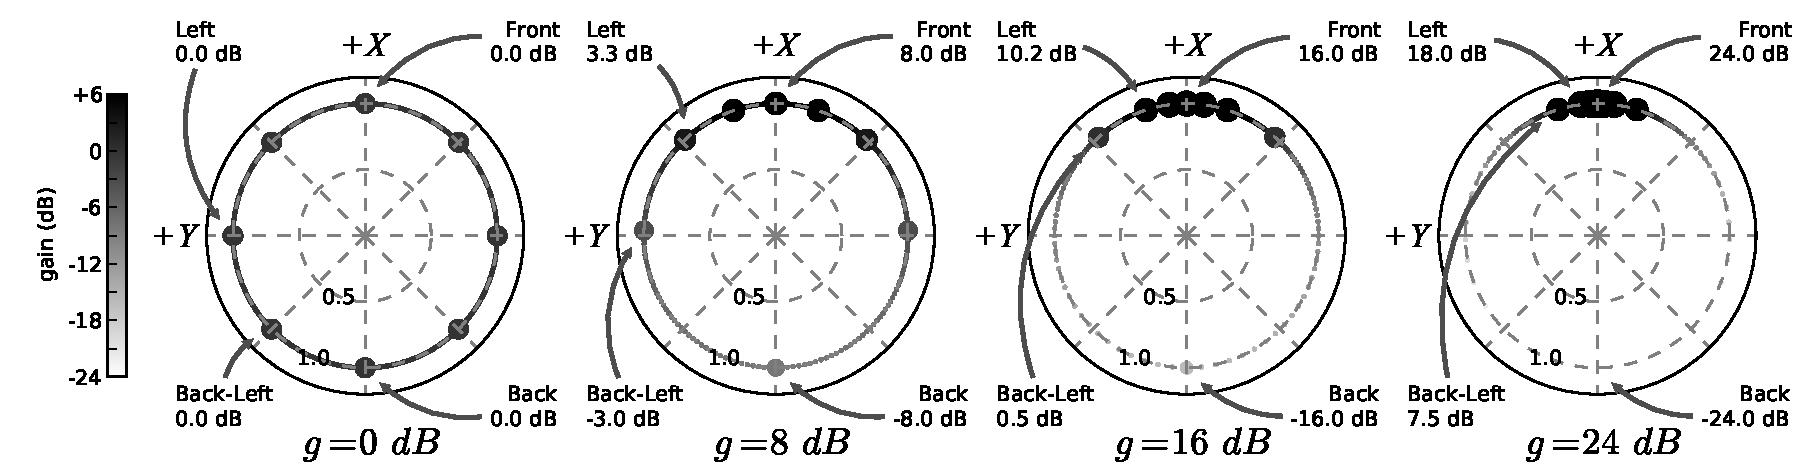
\includegraphics[width=1.\textwidth]{dominance_fig.pdf}
\caption{Dominance}
\label{fig:dominanceFig}
\end{figure}

\begin{figure}
\centering
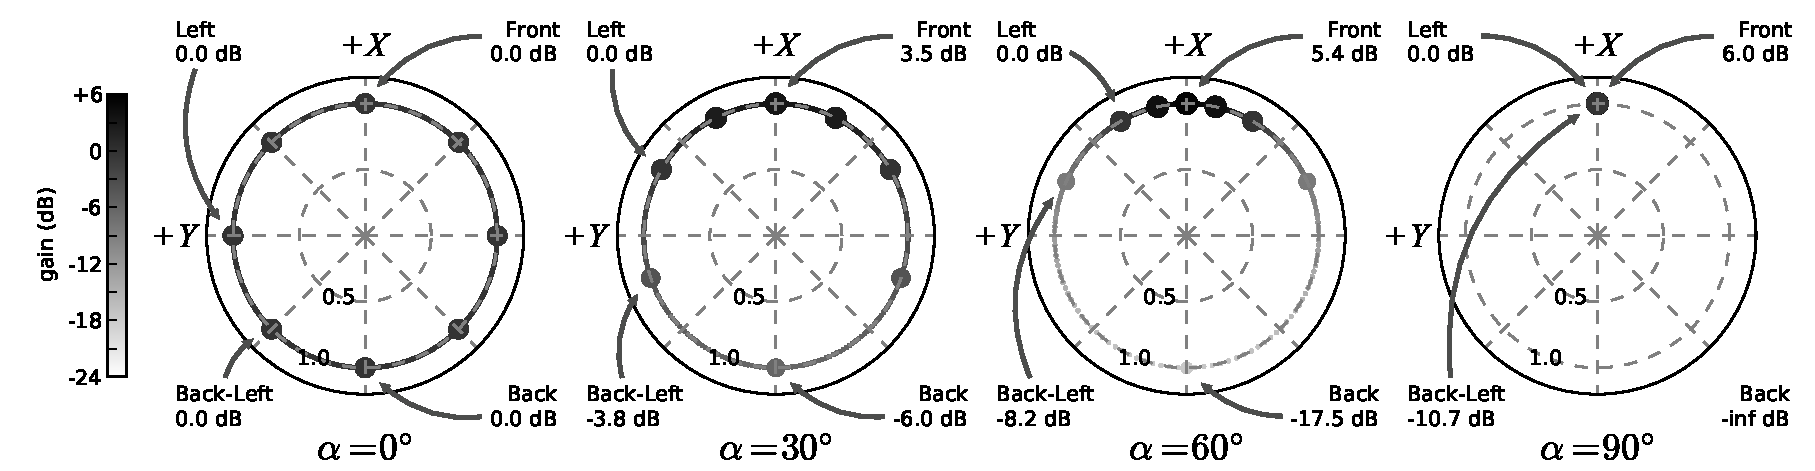
\includegraphics[width=1.\textwidth]{zoom_fig.pdf}
\caption{Zoom}
\label{fig:zoomFig}
\end{figure}

\begin{figure}
\centering
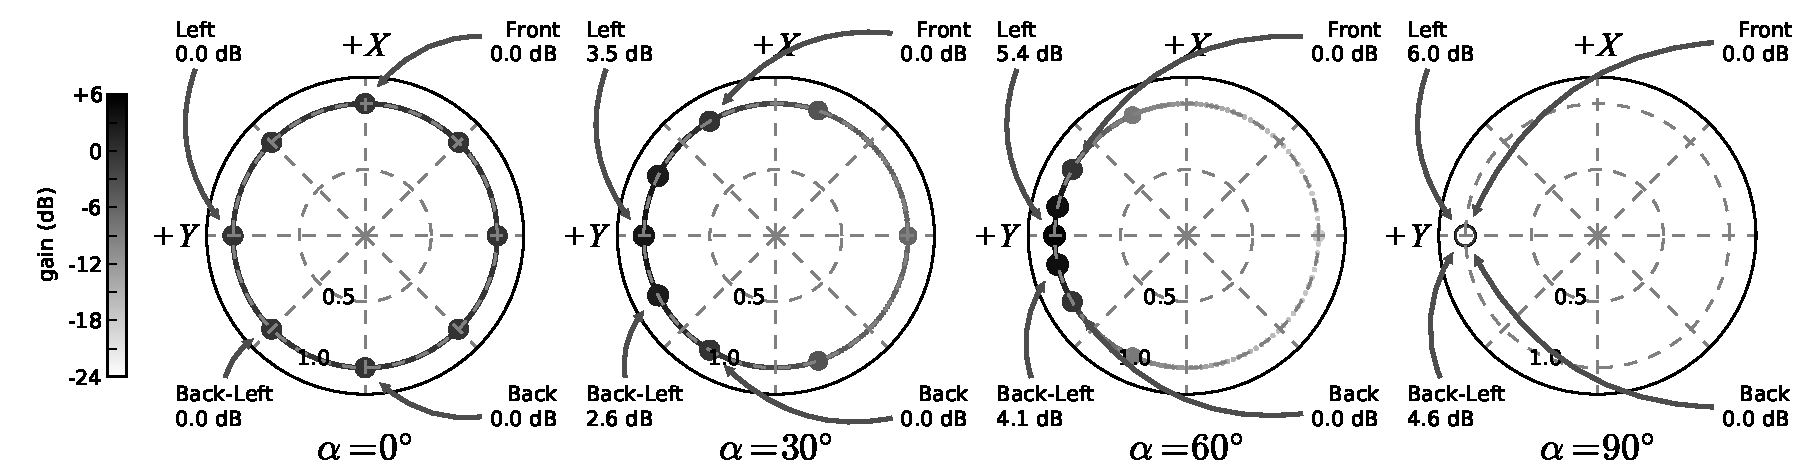
\includegraphics[width=1.\textwidth]{balance_fig.pdf}
\caption{Balance}
\label{fig:balanceFig}
\end{figure}

\begin{figure}
\centering
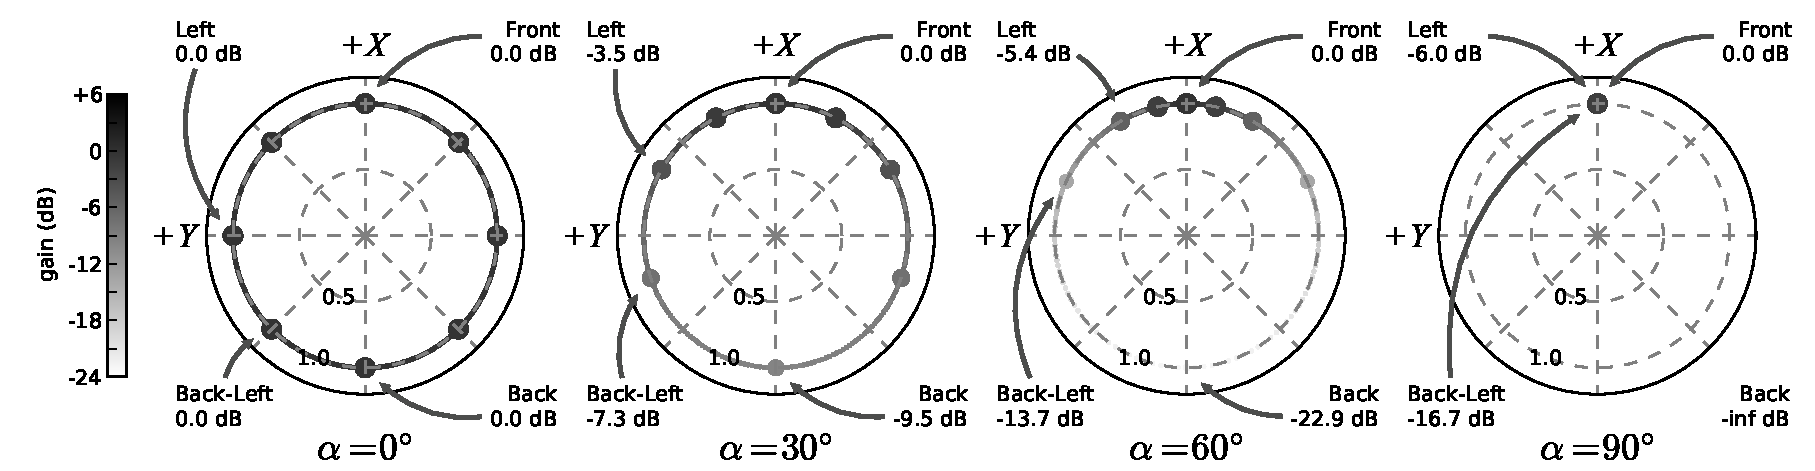
\includegraphics[width=1.\textwidth]{focus_fig.pdf}
\caption{Focus}
\label{fig:focusFig}
\end{figure}

\begin{figure}
\centering
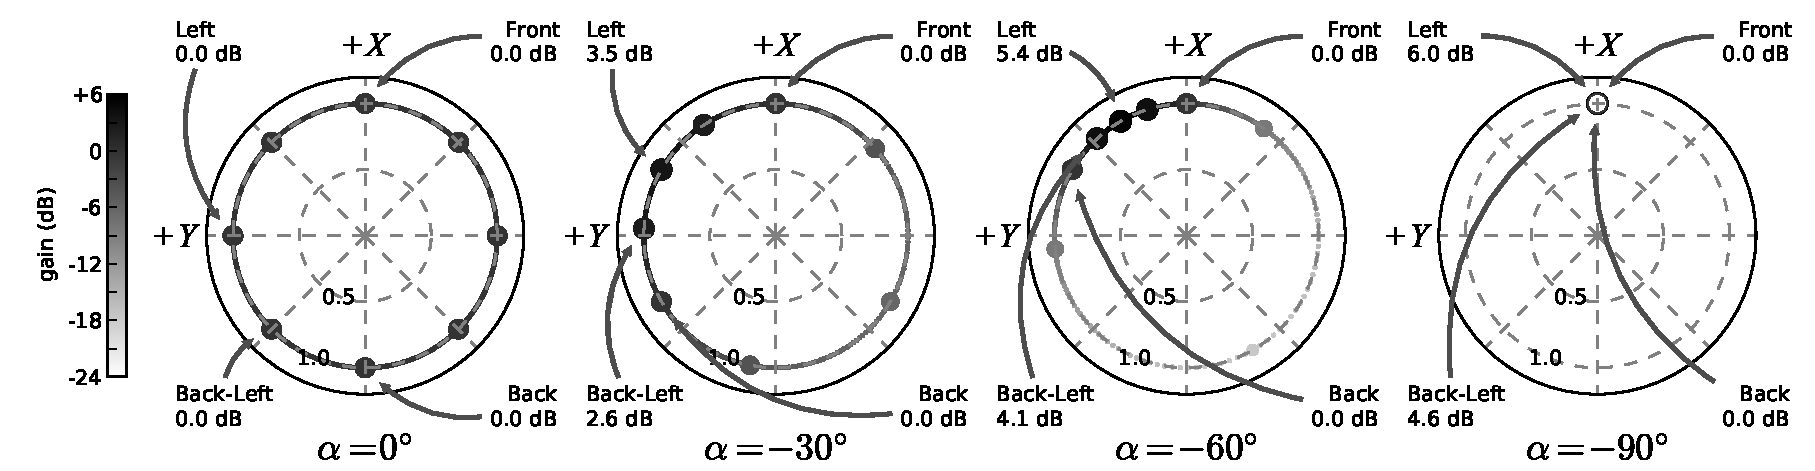
\includegraphics[width=1.\textwidth]{asymmetry_fig.pdf}
\caption{Asymmetry}
\label{fig:asymmetryFig}
\end{figure}

\begin{figure}
\centering
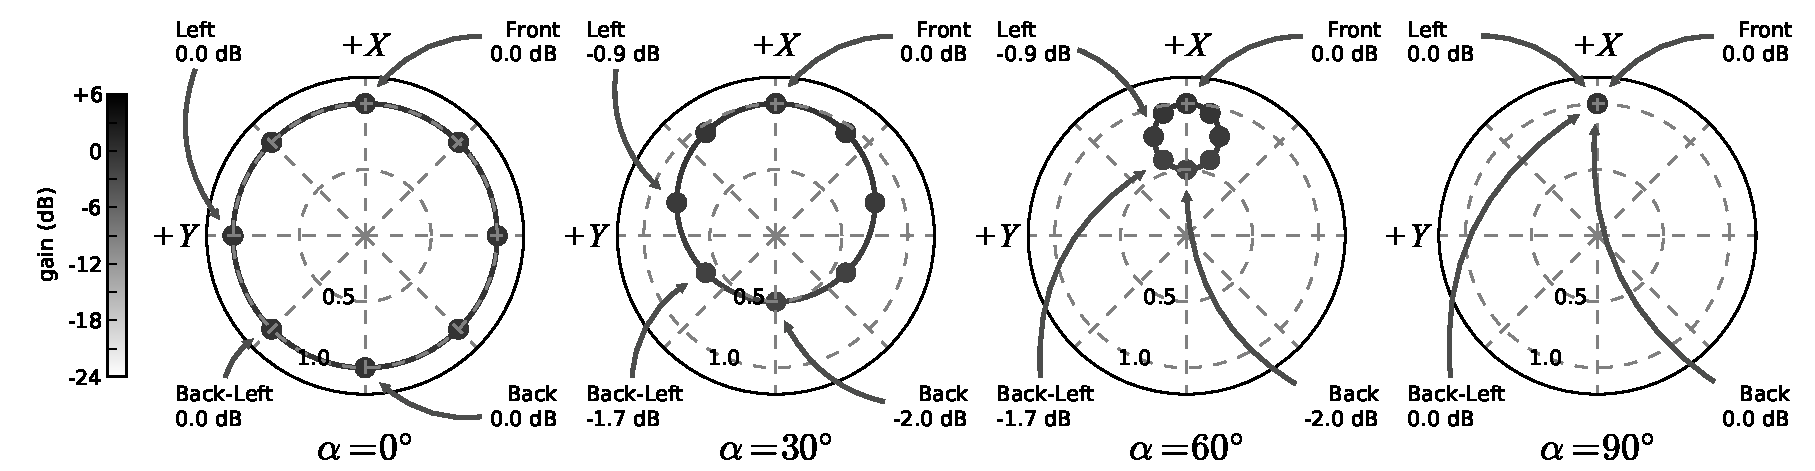
\includegraphics[width=1.\textwidth]{push_fig.pdf}
\caption{Push}
\label{fig:pushFig}
\end{figure}

\begin{figure}
\centering
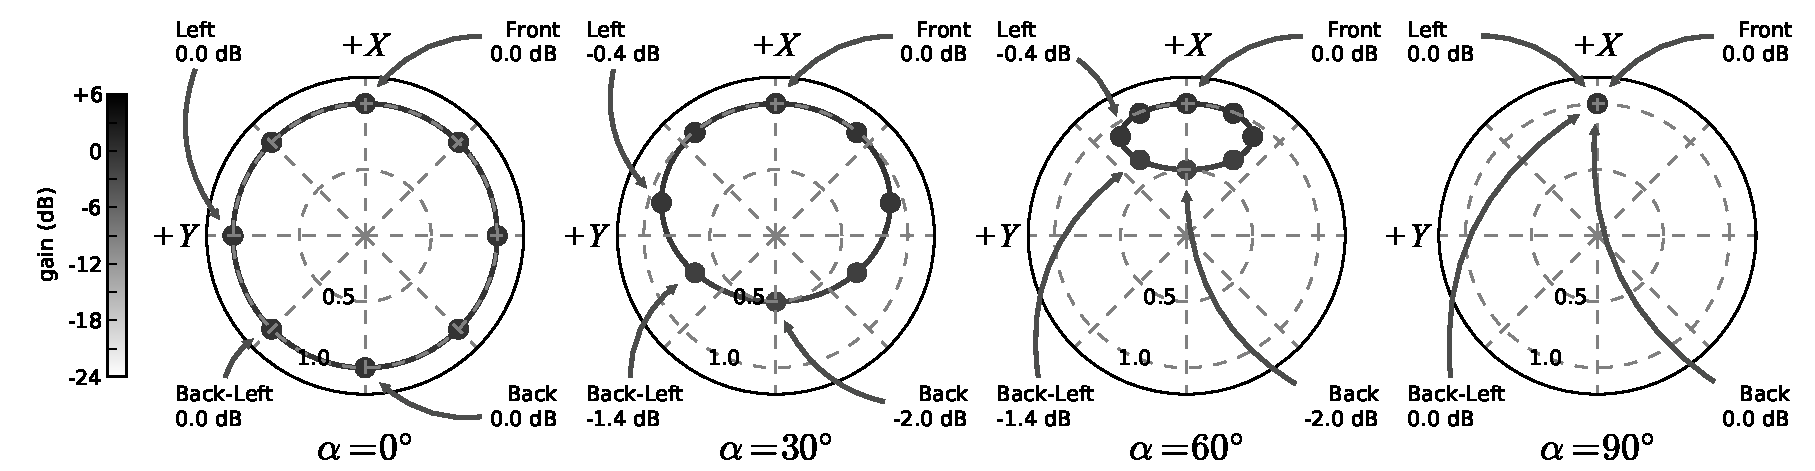
\includegraphics[width=1.\textwidth]{press_fig.pdf}
\caption{Press}
\label{fig:pressFig}
\end{figure}


\end{document}
